\section{評価実験}
\subsection{実験条件の設定}
\subsubsection{モデルの損失関数}
マルチラベル予測の学習のためバイナリ交差エントロピーを用いた。
\subsubsection{モデルの最適化手法}
確率的勾配降下法\cite{SGD}を拡張したAdaptive Moment Estimation (Adam)\cite{Adam}を使用した。
これは勾配の大きさと更新量によって学習率を変化させていく方法で、様々なタスクで高性能を記録している。
\subsubsection{モデルの学習回数とバッチサイズ}
モデルの学習回数はすべて25にした。
これは訓練時における損失関数の推移から判断した。
またバッチサイズはDenseNet121で50、DenseNet161で24、3D-ResNetで3とした。
これは使用した計算機のメモリの容量によって決めた。
\subsection{評価指標}
評価指標は正解率、完全一致正解率、再現率、適合率、F1-Scoreの5つとした。
以下本文中の各データとは、画像を個別に入力する手法では各画像、画像を患者ごとにまとめて入力する手法では画像を時間軸で連結した3次元データを示す。
\subsubsection{正解率 (Acc)}
$各データにおける正解率 = \frac{正解したラベルの数}{マルチラベルにおける全てのラベルの数}$
を計算し、これをすべてのデータにおいて平均を計算した。
\subsubsection{完全一致正解率 (AllAcc)}
$AllAcc=\frac{マルチラベルにおける全てのラベルで一致したデータの数}{全てのデータの数}$
\subsubsection{適合率 (Precision)}
$Precision = \frac{真陽性}{真陽性+偽陽性}$

全てのデータにおける適合率を計算するために、各データにおける混合行列を集計し、その後適合率を計算した。
\subsubsection{再現率 (Recall)}
$Recall = \frac{真陽性}{真陽性+偽陰性}$

全てのデータにおける再現率を計算するために、各データにおける混合行列を集計し、その後再現率を計算した。
\subsubsection{F1-Score}
適合率と再現率がトレードオフの関係であるため、2つの指標を総合的に判断するためにF1-Scoreを用いた。

$F1{\rm \mathchar"712D}Score = \frac{Precision * Recall}{(Precision + Recall) / 2}$

\subsubsection{評価指標とモデルの性能の関係性}
\begin{itemize}
    \item 正解率\\
        正解率は指標としてモデルの性能をあまり評価できない。
        マルチラベル予測の際にこの指標を用いると、マルチラベルのクラス数が多いほど真陰性の割合が多くなり、実際の予測がほとんど行われていなくても高い数値が出るからである。
    \item 完全一致正解率\\
        完全一致正解率は指標としてモデルの性能をあまり評価できない。
        マルチラベル予測の際にこの指標を用いると、マルチラベルのクラス数が多いほど全てを一致させることが困難になり、ほぼ全てのクラスで正解しているもとと全く正解していないものを区別できない。
    \item 適合率\\
        適合率はマルチラベル予測の指標として一般的に用いられる。
        適合率は陽性であると予測したものの中で、実際に陽性であるものの割合である。
        これは本用途においては病変があると予測したものの中で、実際に病変があったものの割合となっており、誤検知の少なさの指標と言える。
    \item 再現率\\
        再現率はマルチラベル予測の指標として一般的に用いられる。
        再現率は実際に陽性であるものの中で、陽性であると予測できたものの割合である。
        これは本用途においては病変があるデータの中で、病変があると予測できたものの割合となっており、見落としの少なさの指標と言える。
    \item F1-Score\\
        F1-Scoreはモデルの性能を最も表していると言える。
        本実験ではこの数値が高いものを良いモデルとして評価する。
\end{itemize}

\subsection{DenseNetを用いた内視鏡画像からの\\マルチラベル予測}
\subsubsection{実験概要}
各画像をマルチラベルと関連付けしたデータセットを用いた。
画像をモデルに入力し出力されたマルチラベルと教師データのマルチラベルから損失を計算し最適化を行った。
モデルが出力したマルチラベルの各ラベルを二値化する際のしきい値を変化させた。
その結果からテスト出力の際のしきい値を決定し、推論を行った。

\subsubsection{実験結果}
結果を表\ref{tb:0}と図\ref{fig:densenet_result}に示す。
表\ref{tb:0}は検証データを用いた際の予測の結果を示す。
この表のTotalは図\ref{fig:multilabel}における全てのラベルにおける結果を、LesionとLabelは図\ref{fig:multilabel}のラベルの1番目と2番目以降に分けて計算した結果を示している。
図\ref{fig:densenet_result_process}は学習過程での損失とF1-Scoreの推移を示している。
図\ref{fig:densenet_result_threshold}はテスト推論において、モデルが出力したマルチラベルの値を二値化する際のしきい値を変化させた際の、PrecisionとRecallとF1-Scoreの変化を示している。

\begin{table}[tb]
    \caption[]{DenseNetを用いた内視鏡画像からの\\マルチラベル予測}
    \label{tb:0}
    \centering
    \normalsize
    \begin{tabular}{c|c|r} \hline
        Total & Acc (\%) & 92.4 \\ \cline{2-3}
         & AllAcc (\%) & 32.8 \\ \cline{2-3}
         & F1-Score (\%) & 73.9 \\ \cline{2-3}
         & Precision (\%) & 88.8 \\ \cline{2-3}
         & Recall (\%) & 63.2 \\ \hline
        Lesion & Acc (\%) & 97.4 \\ \cline{2-3}
         & F1-Score (\%) & 98.7 \\ \cline{2-3}
         & Precision (\%) & 98.0 \\ \cline{2-3}
         & Recall (\%) & 99.4 \\ \hline
        Label & Acc (\%) & 92.1 \\ \cline{2-3}
         & AllAcc (\%) & 34.1 \\ \cline{2-3}
         & F1-Score (\%) & 53.9 \\ \cline{2-3}
         & Precision (\%) & 78.1 \\ \cline{2-3}
         & Recall (\%) & 41.2 \\ \hline
    \end{tabular}
\end{table}
\begin{figure}[tb]
    \centering
        \subfloat[][学習過程]{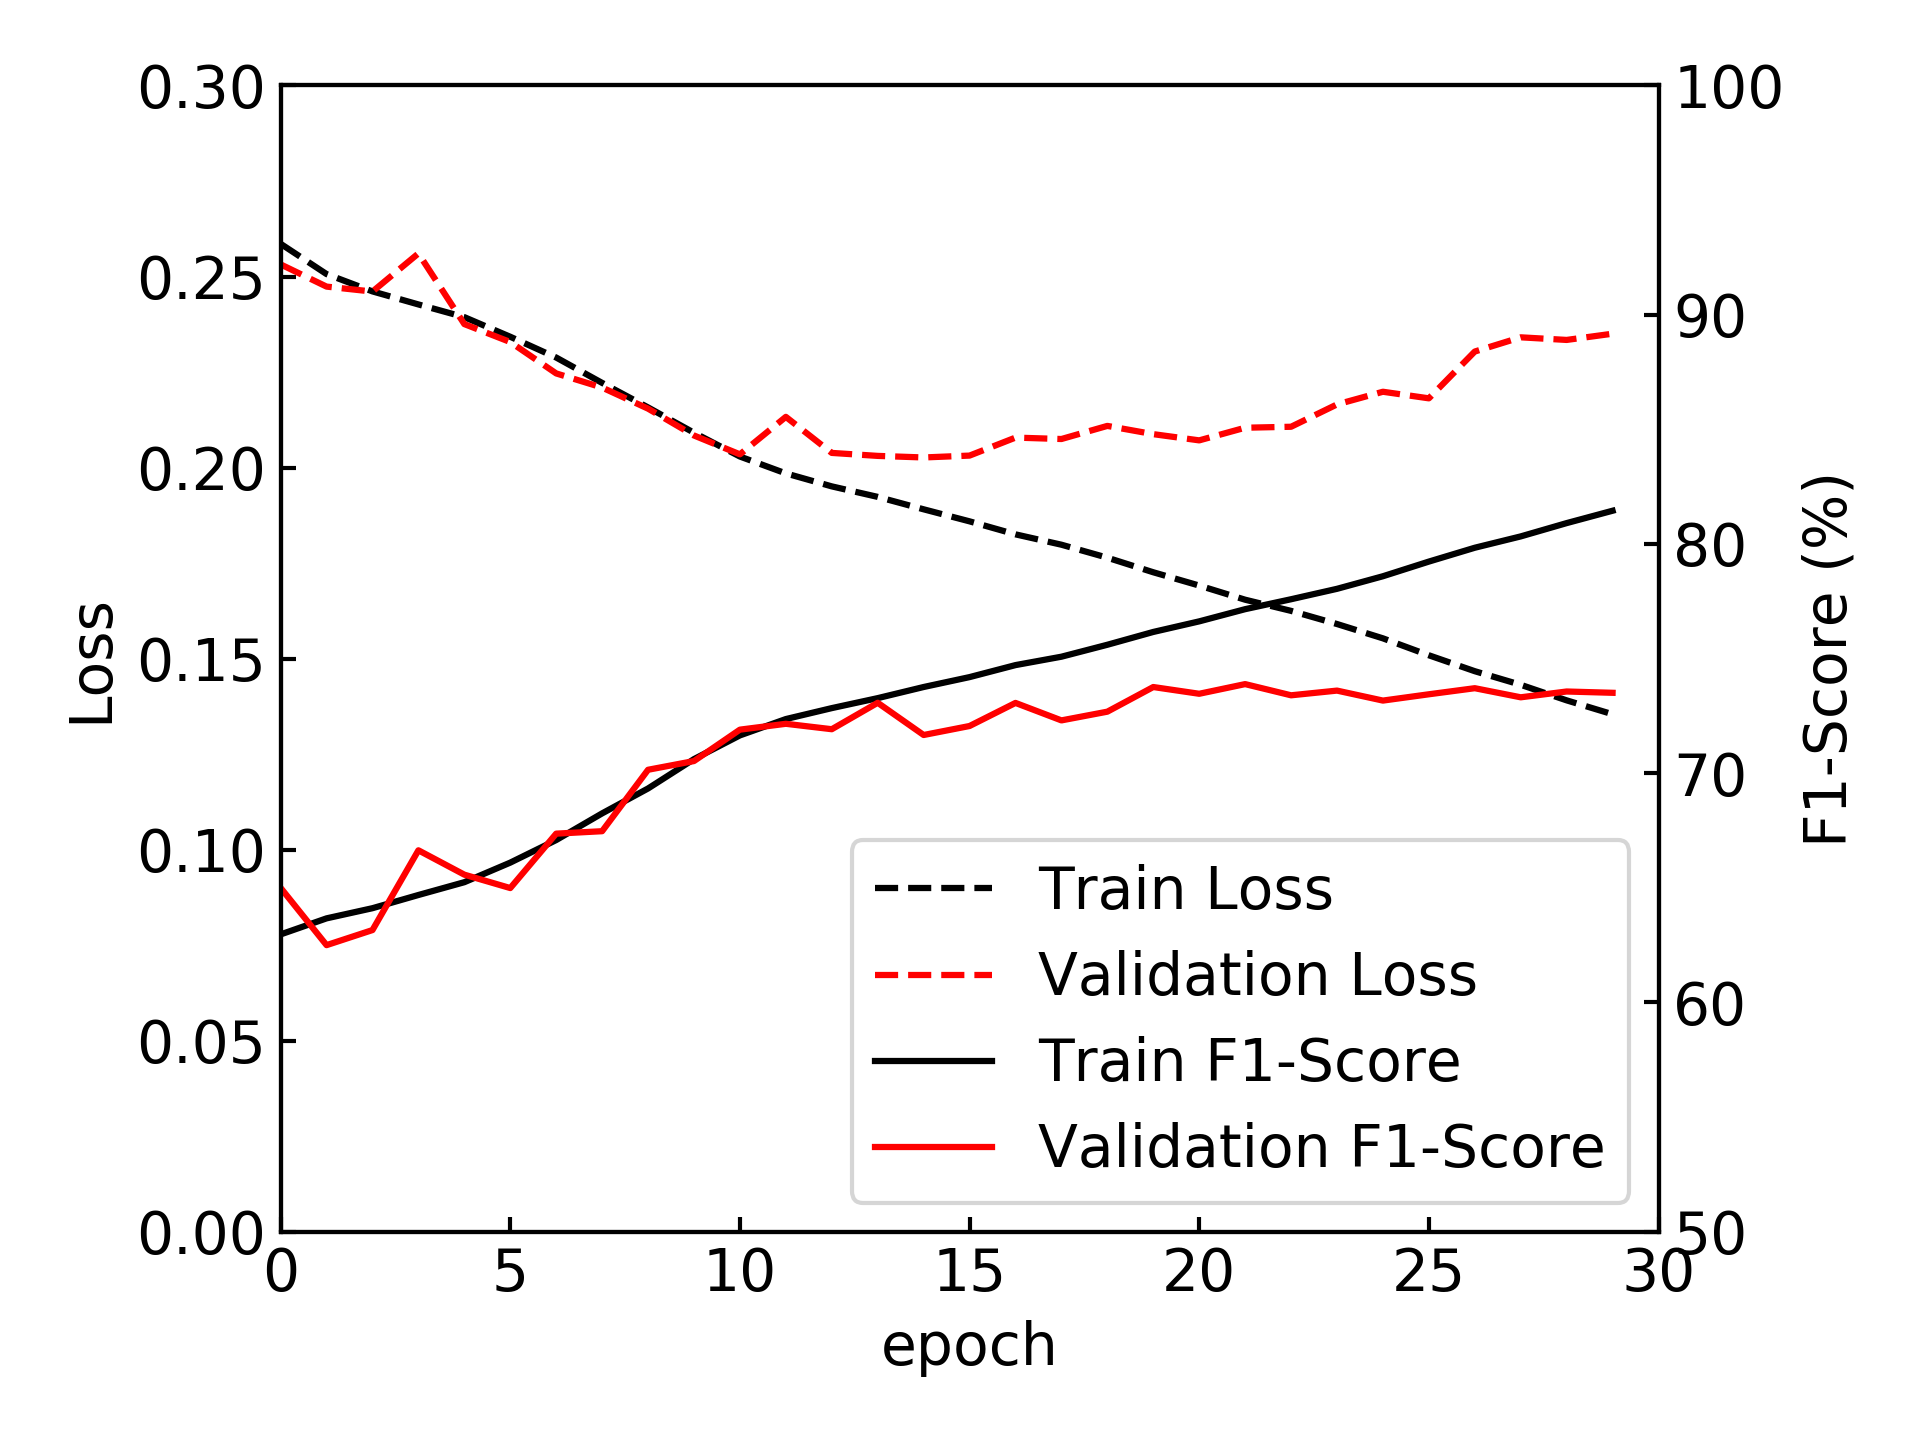
\includegraphics[width=130mm]{./fig/densenet121_e_p02process.png}\label{fig:densenet_result_process}} \quad
        %\subfloat[][検証結果]{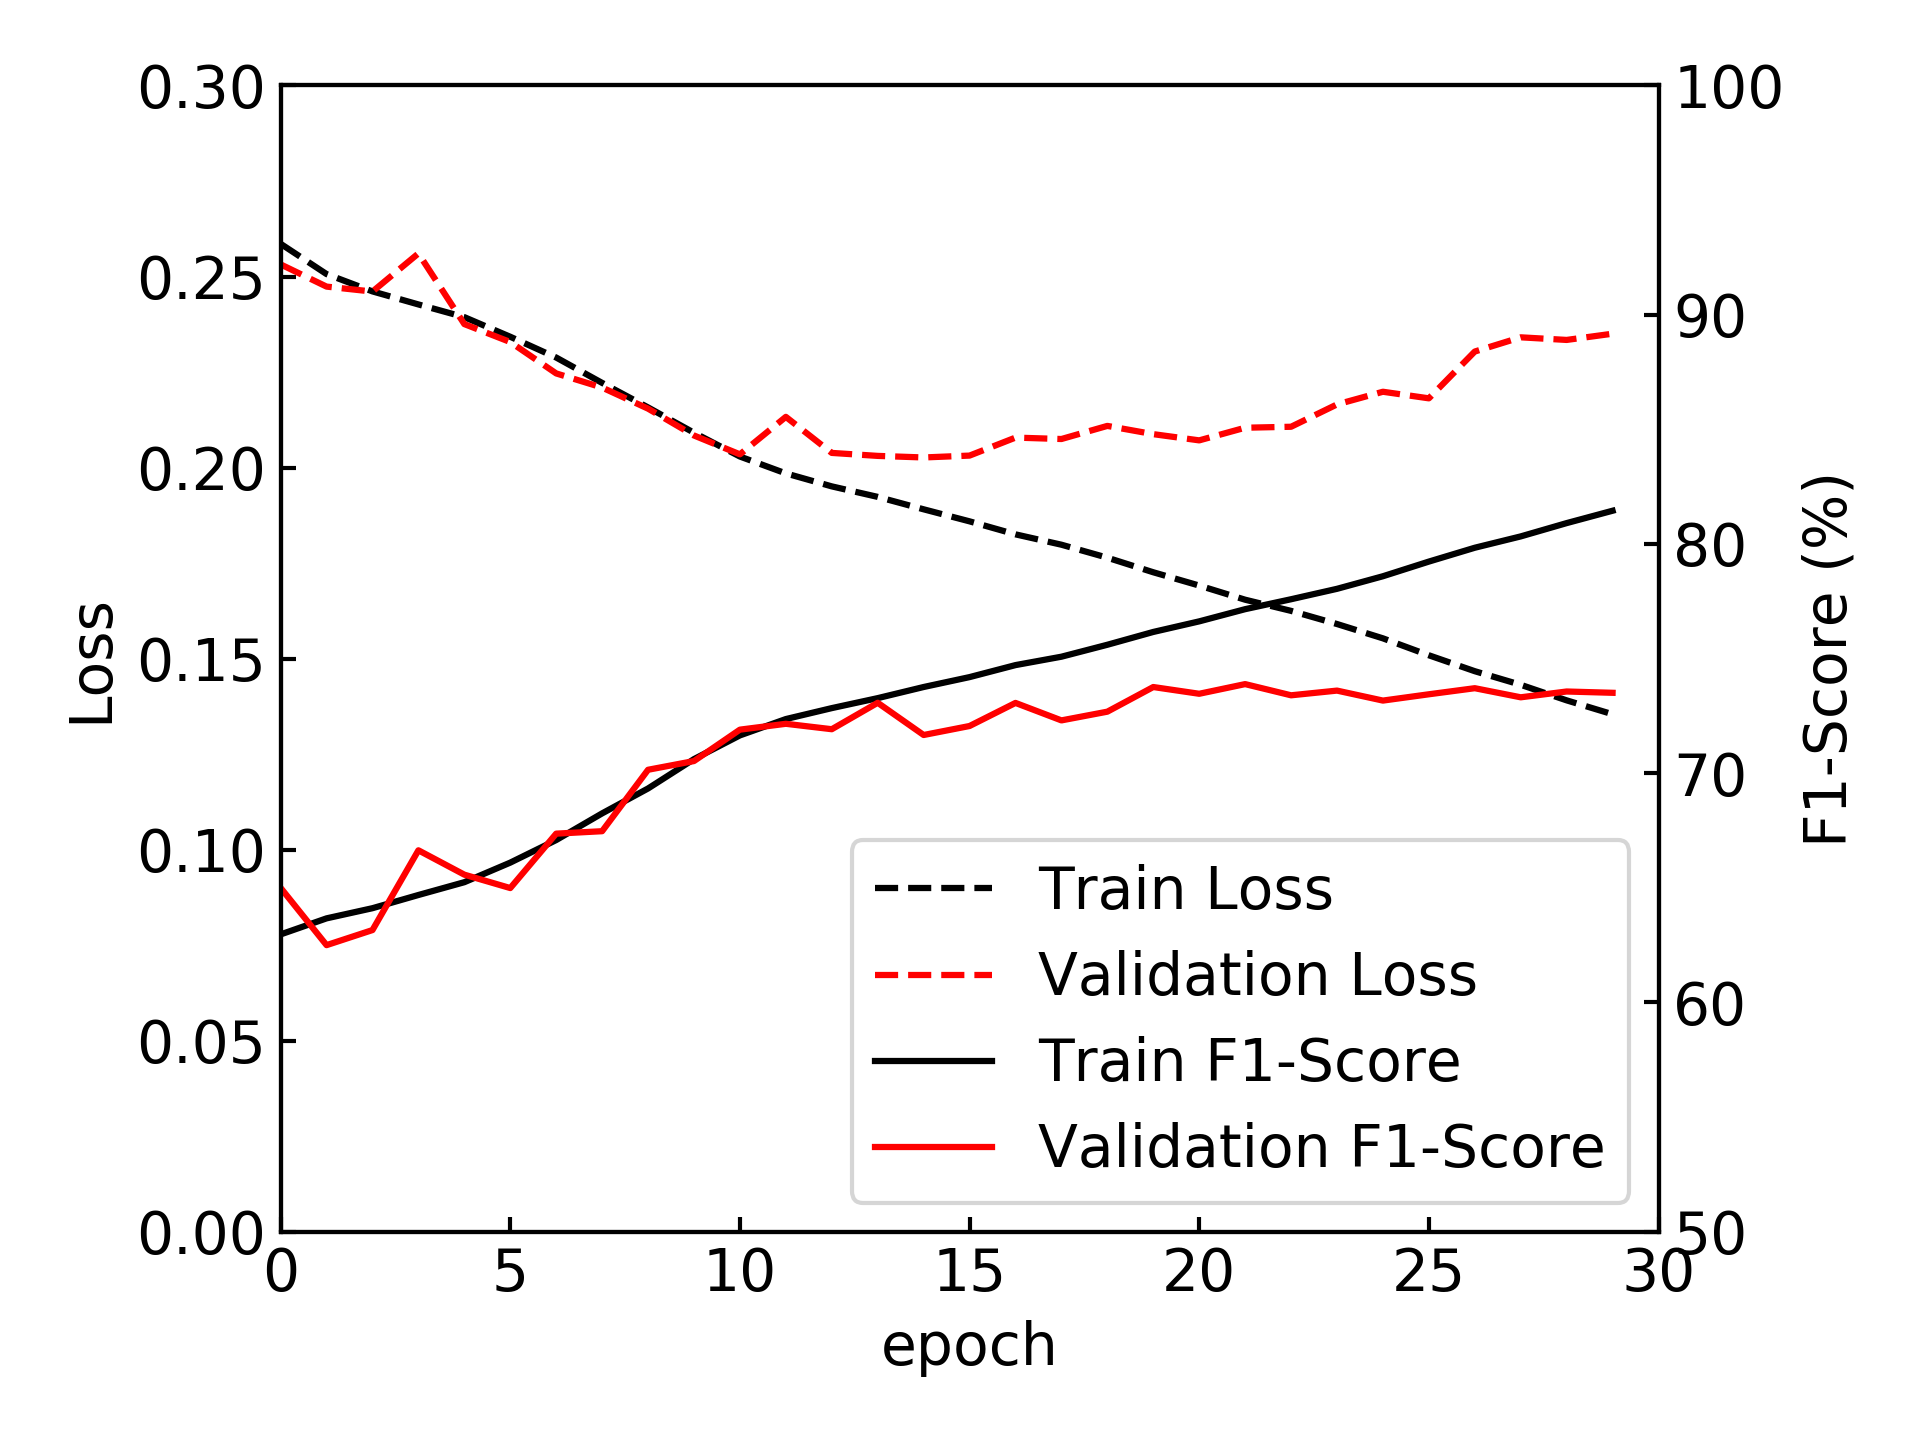
\includegraphics[width=80mm]{./fig/result0.png}\label{fig:0}} \quad
        \subfloat[][各しきい値におけるテスト]{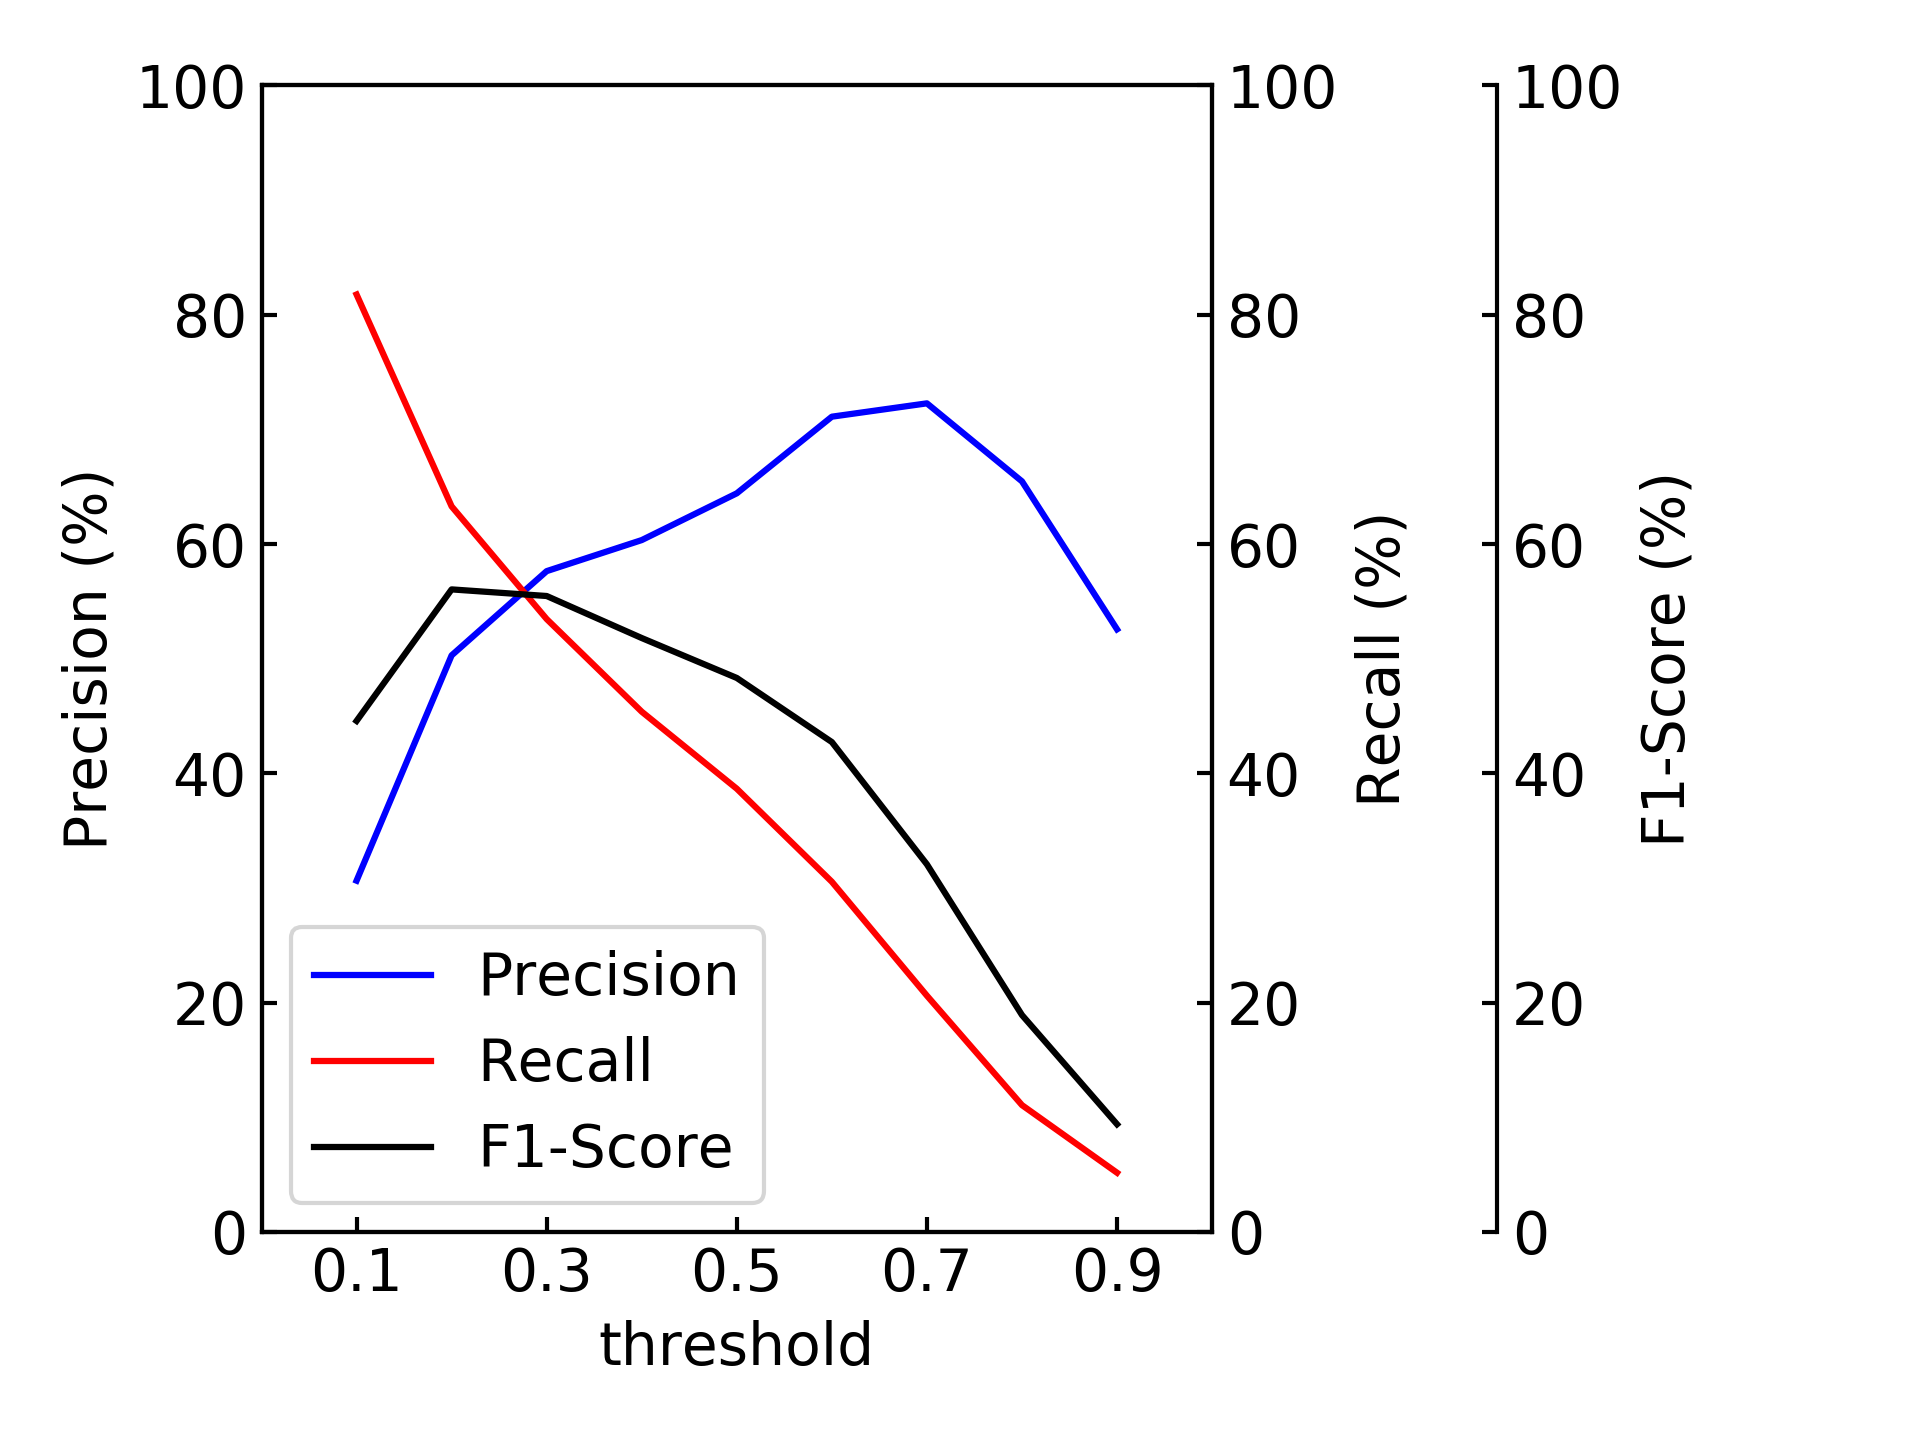
\includegraphics[width=130mm]{./fig/densenet121_e_p02threshold.png}\label{fig:densenet_result_threshold}} \quad
        %\subfloat[][推論結果]{\includegraphics[width=70mm]{./fig/sample4.jpg}\label{fig:04}} \quad
    \captionsetup{format=plain,font=normalsize,margin=30pt,name=図}
    \caption[]{DenseNetを用いた内視鏡画像からのマルチラベル予測}
    \label{fig:densenet_result}
\end{figure}

\subsection{3D-ResNetを用いた内視鏡画像からのマルチラベル予測}
\subsubsection{実験概要}
各患者ごとに画像を時間軸で連結した三次元データとマルチラベルと関連付けしたデータセットを用いた。
三次元データをモデルに入力し出力されたマルチラベルと教師データのマルチラベルから損失を計算し最適化を行った。
モデルが出力したマルチラベルの各ラベルを二値化する際のしきい値を変化させた。
その結果からテスト出力の際のしきい値を決定し、推論を行った。

\subsubsection{実験結果}
結果を表\ref{tb:1}と図\ref{fig:resnet_result}に示す。
表\ref{tb:1}は検証データを用いた際の予測の結果を示す。
この表のTotalは図\ref{fig:multilabel}における全てのラベルにおける結果を、LesionとLabelは図\ref{fig:multilabel}のラベルの1番目と2番目以降に分けて計算した結果を示している。
図\ref{fig:resnet_result_process}は学習過程での損失とF1-Scoreの推移を示している。
図\ref{fig:resnet_result_threshold}はテスト推論において、モデルが出力したマルチラベルの値を二値化する際のしきい値を変化させた際の、PrecisionとRecallとF1-Scoreの変化を示している。

\begin{table}[tb]
    \caption[]{3D-ResNetを用いた内視鏡画像からのマルチラベル予測}
    \label{tb:1}
    \centering
    \normalsize
    \begin{tabular}{c|c|r} \hline
        Total & Acc (\%) & 92.2 \\ \cline{2-3}
         & AllAcc (\%) & 28.5 \\ \cline{2-3}
         & F1-Score (\%) & 72.9 \\ \cline{2-3}
         & Precision (\%) & 86.5 \\ \cline{2-3}
         & Recall (\%) & 63.0 \\ \hline
        Lesion & Acc (\%) & 98.8 \\ \cline{2-3}
         & F1-Score (\%) & 99.4 \\ \cline{2-3}
         & Precision (\%) & 98.9 \\ \cline{2-3}
         & Recall (\%) & 99.9 \\ \hline
        Label & Acc (\%) & 91.7 \\ \cline{2-3}
         & AllAcc (\%) & 28.9 \\ \cline{2-3}
         & F1-Score (\%) & 50.8 \\ \cline{2-3}
         & Precision (\%) & 71.8 \\ \cline{2-3}
         & Recall (\%) & 39.4 \\ \hline
    \end{tabular}
\end{table}
\begin{figure}[tb]
    \centering
        \subfloat[][学習過程]{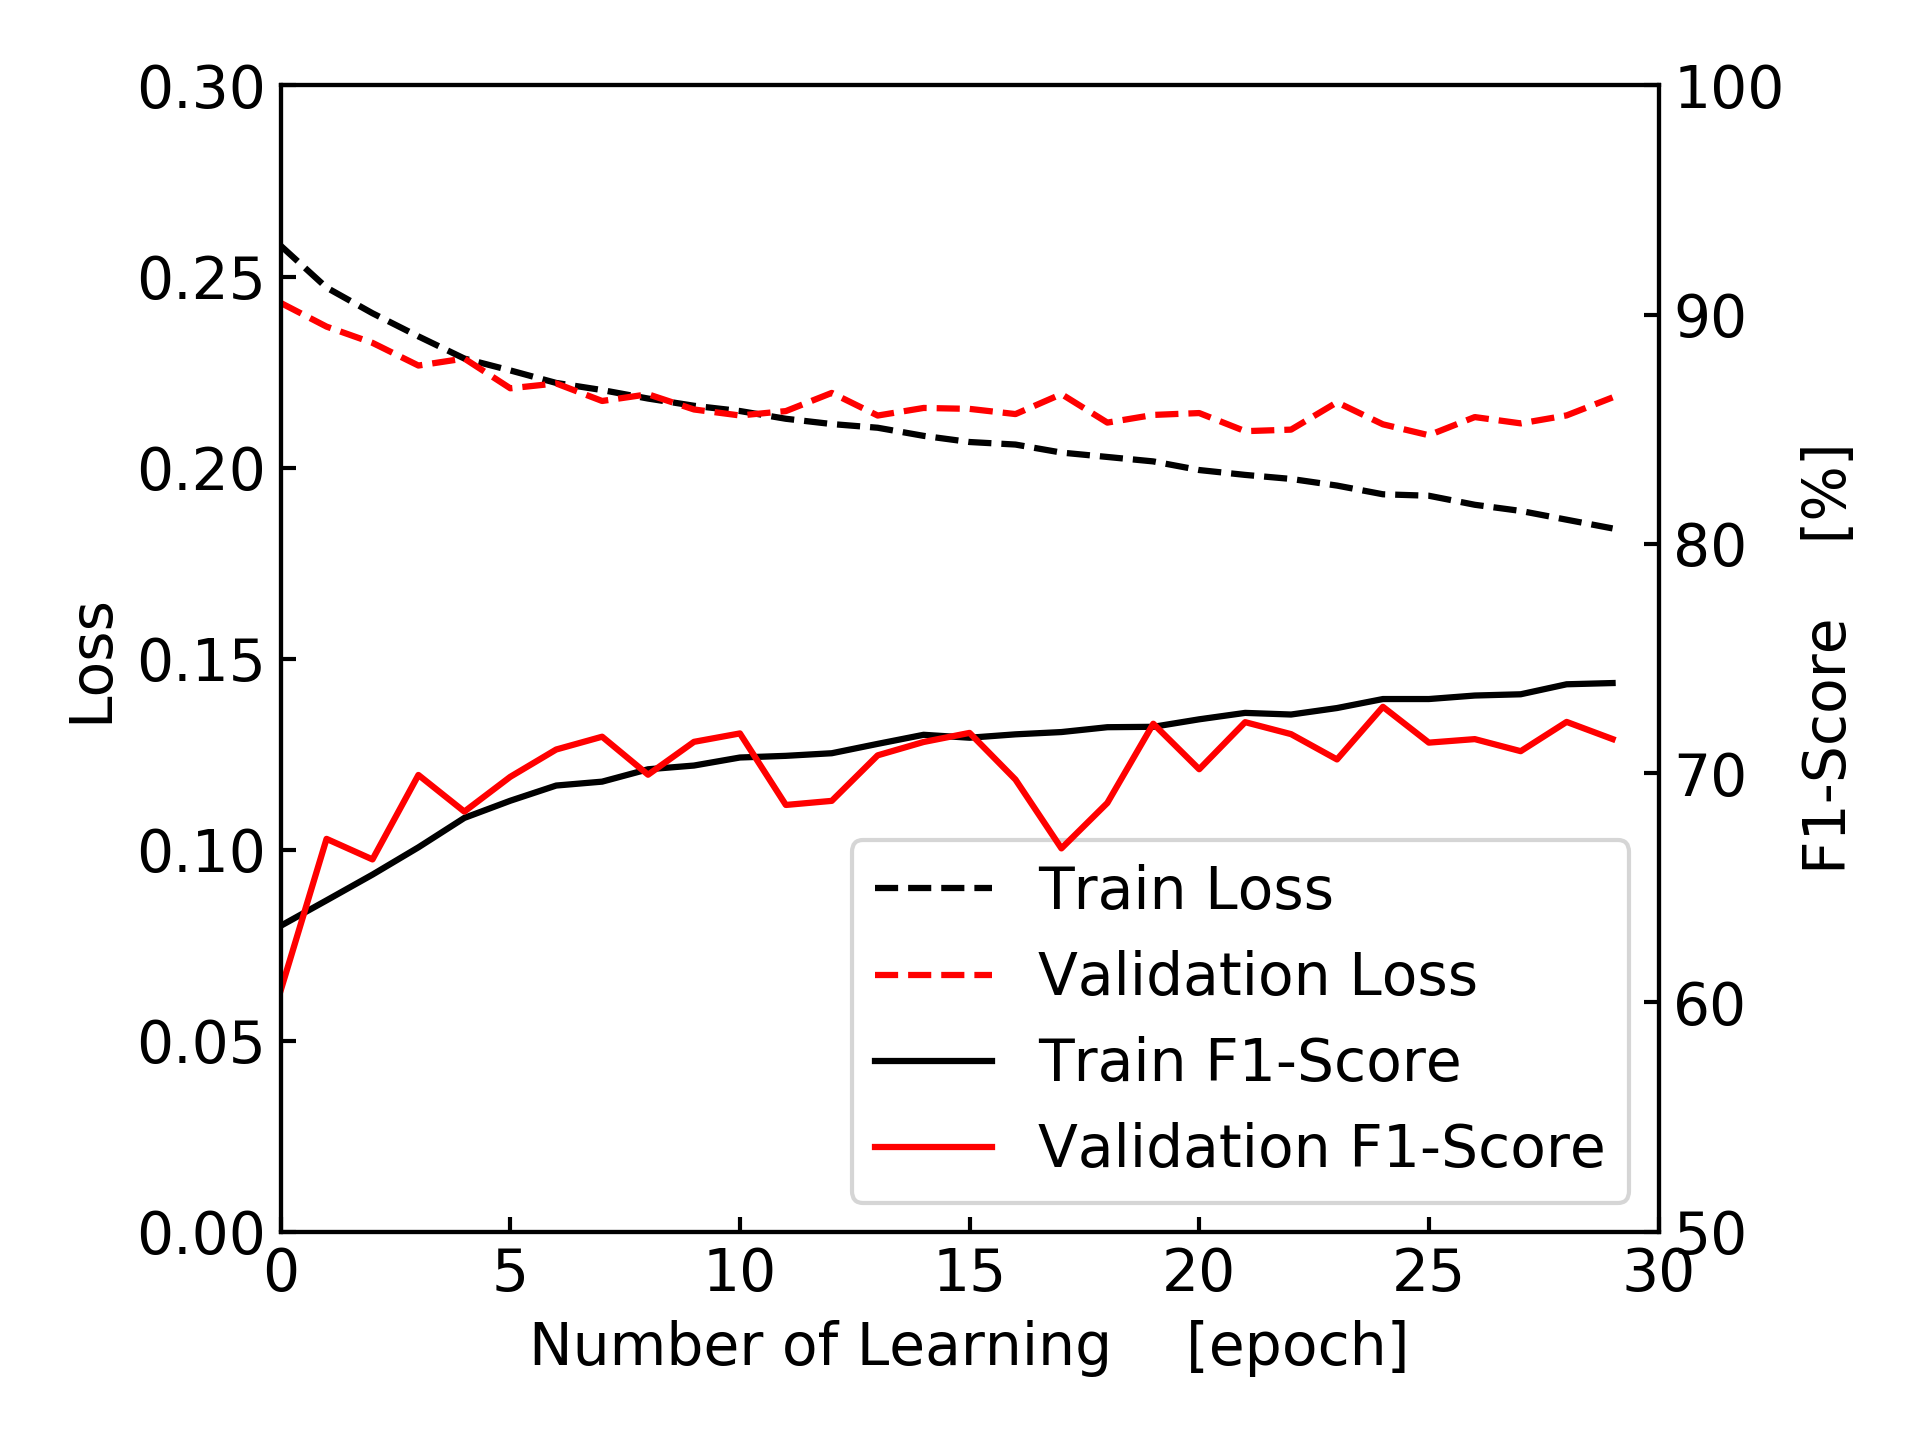
\includegraphics[width=130mm]{./fig/resnet3dprocess.png}\label{fig:resnet_result_process}} \quad
        %\subfloat[][検証結果]{\includegraphics[width=70mm]{./fig/sample2.jpg}\label{fig:02}} \quad
        \subfloat[][各しきい値におけるテスト]{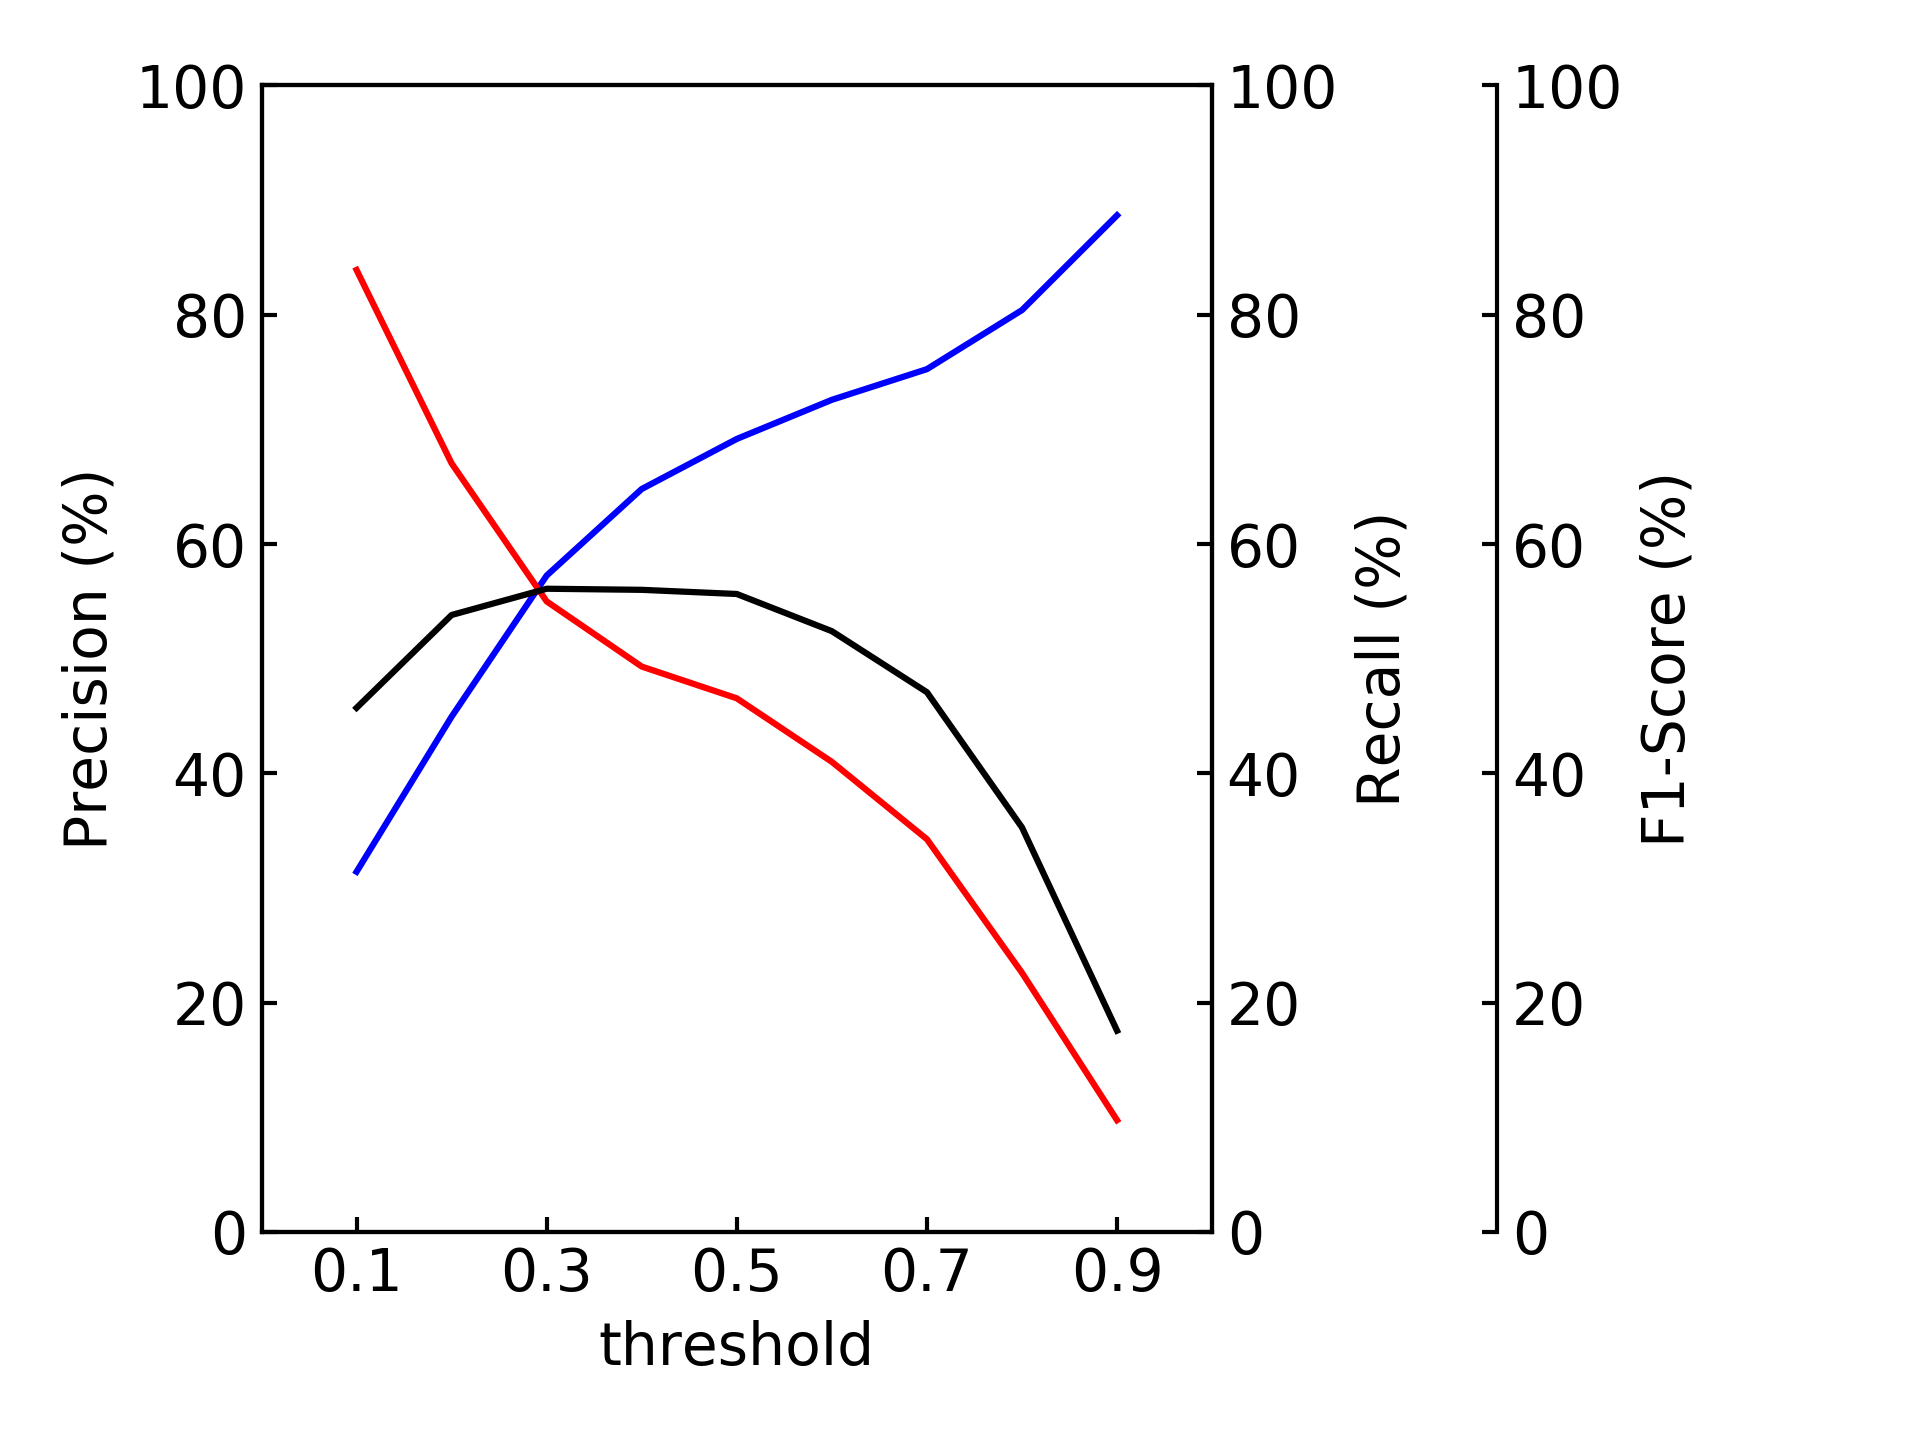
\includegraphics[width=130mm]{./fig/resnet3dthreshold.png}\label{fig:resnet_result_threshold}} \quad
        %\subfloat[][推論結果]{\includegraphics[width=70mm]{./fig/sample4.jpg}\label{fig:04}} \quad
    \captionsetup{format=plain,font=normalsize,margin=30pt,name=図}
    \caption[]{3D-ResNetを用いた内視鏡画像からのマルチラベル予測}
    \label{fig:resnet_result}
\end{figure}
